
%(BEGIN_QUESTION)
% Copyright 2011, Tony R. Kuphaldt, released under the Creative Commons Attribution License (v 1.0)
% This means you may do almost anything with this work of mine, so long as you give me proper credit

Skriv en ligning som beskriver utgangsspenningen som funksjon av temperatur, forutsatt at RTD-en (Resistive Temperature Detector) har en resistans gitt av følgende formel:

$$R_{RTD} = 100 (1 + 0.00392T)$$

$$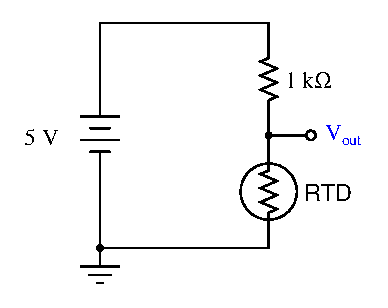
\includegraphics[width=15.5cm]{i00536x01.eps}$$

\vskip 30pt

$V_{out} = f(T) = $

\vfil 

\underbar{file i00536}
\eject
%(END_QUESTION)





%(BEGIN_ANSWER)

Dette er en vurdert oppgave -- ingen svar eller hint oppgis!

%(END_ANSWER)





%(BEGIN_NOTES)

Spenningsdelerformelen gir oss et uttrykk for spenningsfallet over en motstand gitt kildespenning og motstandsverdier:

$$V_{R1} = V_{source} \left(R_1 \over R_1 + R_2 \right)$$

I dette eksemplet er RTD motstanden $R_1$ og den faste 1 k$\Omega$-motstanden er $R_2$, altså:

$$V_{out} = 5 \left(R_{RTD} \over R_{RTD} + 1000 \right)$$

Det vi nå må gjøre er å sette inn RTD-formelen overalt der vi ser $R_{RTD}$ i ligningen over, og deretter forenkle uttrykket:

$$V_{out} = 5 \left(100(1 + 0.00392T) \over 100(1 + 0.00392T) + 1000 \right)$$

$$V_{out} = 5 \left(100 + 0.392T \over 100 + 0.392T + 1000 \right)$$

\vskip 10pt

$$V_{out} = 5 \left({100 + 0.392 T} \over {1100 + 0.392 T}\right)$$

%INDEX% Matematikkrepetisjon: innsetting av ligninger

%(END_NOTES)

